\documentclass[12pt]{article}
\usepackage[utf8]{inputenc}
\usepackage{kotex}
\usepackage{graphicx}
\usepackage{subfigure}
\usepackage{titling}
\setlength{\droptitle}{-2cm}
\usepackage{array}
\usepackage{amssymb}
\usepackage{amsmath}
\usepackage{siunitx} 
\usepackage{enumerate} 
\usepackage{pgfplots}
\usepackage{pgfplotstable}
\usepackage{tikz,pgfplots}
\usepackage{wasysym}
\usepackage{geometry}
\usepackage{authblk}
\usepackage{kotex}
\usepackage{bibunits}
\usepackage{tabularx}
\usepackage{hyperref}
\usepackage{chngcntr}
\counterwithin*{subsection}{section}
\renewcommand{\thesubsection}{\thesection.\alph{subsection}}

\geometry{
    a4paper,
    total={170mm,257mm},
    left=20mm,
    top=20mm,
}

\title{\textbf{Artificial Intelligence: HW 3}}
\author{Jeong Min Lee}

\begin{document}
\maketitle

\section{Linear Regression}
\subsection{}
Let $f$ be the target function. I'll use the superscript with parenthesis to describe the n-th sample vector.
\begin{equation}
    f(\boldsymbol{\omega},\overline{\boldsymbol{x}^{(n)}}) = \sum_n\frac{1}{2}\left(t^{(n)} - \boldsymbol{\omega}^T \overline{\boldsymbol{x}^{(n)}}\right)^2
\end{equation}

To minimize $f$, differentiate it by $\boldsymbol{\omega}$ and find the $\boldsymbol{\omega}_0$ which makes the derivative zero. To make expression simple, I used the Einstein notation. 

\begin{align*}
    {\partial f \over \partial \omega_j} &= -(t^{(n)} - \boldsymbol{\omega}^T \overline{\boldsymbol{x}^{(n)}}) \cdot {\partial \over \partial \omega_j} \boldsymbol{\omega}^T \bar{\boldsymbol{x}}^{(n)} \\
    &= -(t^{(n)} - \boldsymbol{\omega}^T \overline{\boldsymbol{x}^{(n)}}) x_j^{(n)}\\
    &=0
\end{align*}

By enumerating the ${\partial f \over \partial \omega_j}$ horizontally, one can get ${\partial f \over \partial \boldsymbol{\omega}}$.

\begin{equation}
    \sum_n t^{(n)}\begin{pmatrix} x^{(n)}_1 \\ \vdots \\ x^{(n)}_M \end{pmatrix}^T = \sum_n \begin{pmatrix} \boldsymbol{\omega}^T \overline{\boldsymbol{x}^{(n)}}x_1^{(n)} \\ \vdots \\ \boldsymbol{\omega}^T \overline{\boldsymbol{x}^{(n)}}x_M^{(n)} \end{pmatrix}^T
\end{equation}

The left hand side is simply $\sum_n t^{(n)}\overline{\boldsymbol{x}^{(n)}}^T$. From the linearity of vector summation rule, the right hand side is $\left(\left(\sum_n \overline{\boldsymbol{x}^{(n)}} \cdot \overline{\boldsymbol{x}^{(n)}}^T\right)\boldsymbol{\omega}\right)^T$.
By taking transpose to both sides, one can get the following equation.

\begin{equation}
    \left[\sum_n \overline{\boldsymbol{x}^{(n)}} \cdot \overline{\boldsymbol{x}^{(n)}}^T\right] \boldsymbol{\omega} = \sum_n t^{(n)}\overline{\boldsymbol{x}^{(n)}}
\end{equation}

Therefore, $\boldsymbol{A} = \sum_n \overline{\boldsymbol{x}^{(n)}} \cdot \overline{\boldsymbol{x}^{(n)}}^T$ and $\boldsymbol{b} = \sum_n t^{(n)} \overline{\boldsymbol{x}^{(n)}}$

\subsection{}
$\overline{\boldsymbol{x}^{(1)}} = (1,0)^T, t^{(1)} = 1.$ $\overline{\boldsymbol{x}^{(2)}} = (1,\epsilon)^T, t^{(2)} = 1.$ 
$\boldsymbol{A} = \overline{\boldsymbol{x}^{(1)}} \cdot \overline{\boldsymbol{x}^{(1)}}^T + \overline{\boldsymbol{x}^{(1)}} \cdot \overline{\boldsymbol{x}^{(2)}}^T = \begin{pmatrix}
2 & \epsilon \\ \epsilon & \epsilon^2
\end{pmatrix}$
$\boldsymbol{b} = \overline{\boldsymbol{x}^{(1)}} + \overline{\boldsymbol{x}^{(2)}} = (2,\epsilon)^T$. Since $\boldsymbol{A}$ is invertible(determinant is nonzero.), 

\begin{align}
    \boldsymbol{\omega} &= \boldsymbol{A}^{-1}\boldsymbol{b} \\ &= \frac{1}{\epsilon^2} \begin{pmatrix}
        \epsilon^2 & -\epsilon \\ -\epsilon & 2
        \end{pmatrix} \begin{pmatrix} 2 \\ \epsilon \end{pmatrix} \\ &= \begin{pmatrix} 1 \\ 0 \end{pmatrix}
\end{align}

\subsection{}
$\boldsymbol{A}$ is same to the above one. $\boldsymbol{b} = (1+\epsilon)\cdot \overline{\boldsymbol{x}^{(1)}} + \overline{\boldsymbol{x}^{(2)}} = (2 + \epsilon,\epsilon)^T $

\begin{align}
    \boldsymbol{\omega} &= \boldsymbol{A}^{-1}\boldsymbol{b} \\ &= \frac{1}{\epsilon^2} \begin{pmatrix}
        \epsilon^2 & -\epsilon \\ -\epsilon & 2
        \end{pmatrix} \begin{pmatrix} 2 + \epsilon \\ \epsilon \end{pmatrix} \\ &= \begin{pmatrix} 1+\epsilon \\ -1 \end{pmatrix}
\end{align}

\subsection{}
$\boldsymbol{\omega}_{b} = (1,0)^T, \boldsymbol{\omega}_{c} = (1.1,-1)^T$.
The difference of $\Delta \boldsymbol{\omega} = \boldsymbol{\omega}_{c} - \boldsymbol{\omega}_{b} =(\epsilon,-1)^T = (0.1,-1)^T$ 


\section{Linear Regression with Regularization}
\subsection{}
$\textbf{Claim 1} : \boldsymbol{A}$ is positive semi-definite.

\noindent\textbf{proof}

$\boldsymbol{A}$ is trivially symmetry matrix. $\forall \boldsymbol{v} \in \mathbb{R}^n, \boldsymbol{v}^T \boldsymbol{A} \boldsymbol{v} = \sum_n \boldsymbol{v}^T \overline{\boldsymbol{x}^{(n)}} \cdot \overline{\boldsymbol{x}^{(n)}}^T \boldsymbol{v} = \sum_n \lVert\boldsymbol{v}^T \overline{\boldsymbol{x}^{(n)}} \rVert^2 \ge 0._\blacksquare$
\\

\noindent$\textbf{Claim 2} : \boldsymbol{A}\boldsymbol{x} = \lambda \boldsymbol{x} \iff \boldsymbol{A}^{-1}\boldsymbol{x} = \lambda^{-1} \boldsymbol{x}$ where $\lambda \ne 0$ and $\boldsymbol{A}$ is invertible. 

\noindent\textbf{proof}

$\boldsymbol{A}\boldsymbol{x} = \lambda \boldsymbol{x} \iff \boldsymbol{A}^{-1}\boldsymbol{A}\boldsymbol{x} = \lambda \boldsymbol{A}^{-1}\boldsymbol{x} \iff \lambda^{-1} \boldsymbol{x} = \boldsymbol{A}^{-1} \boldsymbol{x}._\blacksquare$
\\

\noindent
Let S(A) be the set of all eigenvalues of A.
\begin{equation}
    S(\boldsymbol{A}) \equiv \left\{\lambda_i | \text{for some } \boldsymbol{x} \in \mathbb{R},\; \boldsymbol{A}\boldsymbol{x} = \lambda_i \boldsymbol{x} \right\}
\end{equation}

\noindent
For $\forall \tilde{\lambda} \in S(\boldsymbol{A}+\lambda \boldsymbol{I}), (\boldsymbol{A}+\lambda I)\boldsymbol{x} = \tilde{\lambda}\boldsymbol{x}.$ 

\noindent
By multiplying $\boldsymbol{x}^T, \boldsymbol{x}^T (\boldsymbol{A} + \lambda \boldsymbol{I}) \boldsymbol{x} =  \boldsymbol{x}^T \boldsymbol{A} \boldsymbol{x} + \lambda = \tilde{\lambda} \ge \lambda.(\because \boldsymbol{A} \text{ is positive semi-definite.})$

\noindent
This implies that $\min(S(\boldsymbol{A}+\lambda \boldsymbol{I})) \ge \lambda$. Equivalently,due to the \textbf{Claim 2}, this also means that $\max(S((\boldsymbol{A} + \lambda I)^{-1})) \le \lambda^{-1}$. By noticing that $\max(S((\boldsymbol{A} + \lambda I)^{-1})) = \rho((\boldsymbol{A} + \lambda I)^{-1})$, the proof is done. Note that for the equality, $\boldsymbol{A}\boldsymbol{x} = \textbf{0}$ must have nontrivial solution. 

\subsection{}
For both problems, the $\boldsymbol{A} + \lambda \boldsymbol{I}$ is following. 

\begin{equation}
    \boldsymbol{A} + \lambda \boldsymbol{I} = \begin{pmatrix}
        2 + \lambda & \epsilon \\ \epsilon & \epsilon^2 + \lambda
    \end{pmatrix}
    \label{eqn:A}
\end{equation}

Since (\ref{eqn:A}) is invertible, one can get $\boldsymbol{\omega_b}, \boldsymbol{\omega_c}$. 

\begin{align*}
    \boldsymbol{\omega_b} &= \frac{1}{(1+\lambda)\epsilon^2 + \lambda(\lambda + 2)} \cdot \begin{pmatrix}
        \epsilon^2 + \lambda & - \epsilon \\ - \epsilon & 2 + \lambda
    \end{pmatrix} \cdot \begin{pmatrix}
        2 \\ \epsilon
    \end{pmatrix}\\
    &= \frac{1}{(1+\lambda)\epsilon^2 + \lambda(\lambda + 2)} \cdot \begin{pmatrix}
        \epsilon^2 + 2\lambda \\ \epsilon\lambda
    \end{pmatrix} \\
    &= \begin{pmatrix}
        0.973\\ 0.044
    \end{pmatrix}
\end{align*}

\begin{align*}
    \boldsymbol{\omega_c} &= \frac{1}{(1+\lambda)\epsilon^2 + \lambda(\lambda + 2)} \cdot \begin{pmatrix}
        \epsilon^2 + \lambda & - \epsilon \\ - \epsilon & 2 + \lambda
    \end{pmatrix} \cdot \begin{pmatrix}
        2 + \epsilon \\ \epsilon
    \end{pmatrix}\\
    &= \frac{1}{(1+\lambda)\epsilon^2 + \lambda(\lambda + 2)} \cdot \begin{pmatrix}
        \epsilon^3 + \epsilon^2 +\lambda \epsilon + 2 \lambda \\ -\epsilon^2 + \lambda\epsilon
    \end{pmatrix} \\
    &= \begin{pmatrix}
        1.026 \\ -0.044
    \end{pmatrix}
\end{align*}

Furthemore, $\Delta \boldsymbol{\omega} = \boldsymbol{\omega_c} - \boldsymbol{\omega_b}$ can be obtained. 

\begin{equation}
    \Delta \boldsymbol{\omega} = \frac{1}{(1+\lambda)\epsilon^2 + \lambda(\lambda + 2)} \begin{pmatrix}
        \epsilon^3 + \lambda\epsilon \\ -\epsilon^2
    \end{pmatrix} = \begin{pmatrix}
        0.0531 \\ -0.088
    \end{pmatrix}
\end{equation}

\subsection{}
One can notice that $\lVert\Delta \boldsymbol{\omega}\rVert$ with regularization is much smaller than $\lVert\Delta \boldsymbol{\omega}\rVert$ without regularization. This implies that regularization makes the parameters less variable with respect to small noise in input data. This can be verified by the following figure.

\begin{figure}[!h]
    \centering
    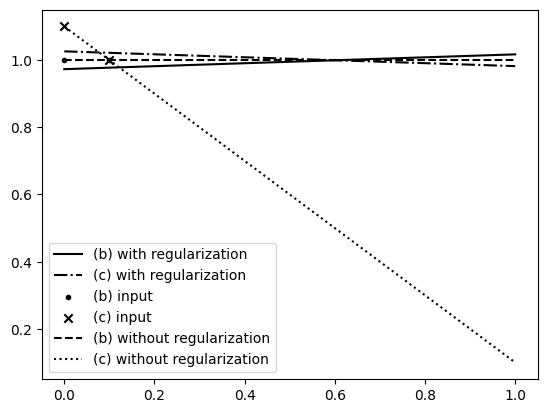
\includegraphics[scale = 0.5]{./figures/output2.png}
    \caption{The linear regression result of (b) and (c)}
    \label{fig:regularization}
\end{figure}

According to the figure \ref{fig:regularization}, the linear regression with regularization tends to be stable for the noised sample (c) and unnoised sample (b). However, the regression without the regularization has more fluctuation for noised sample. 

\section{LR with Regularization: A Probabilistic Perspective}
The Gaussian prior implies the following.
\begin{align*}
    \text{Pr}(\boldsymbol{\omega}) = \mathcal{N}(\boldsymbol{0},\frac{1}{\lambda} \boldsymbol{I}) = \frac{\lambda^{N/2}}{2\pi^{N/2}}\exp\left({-\frac{1}{2}\boldsymbol{\omega}^T \lambda \boldsymbol{\omega}}\right)
\end{align*}

\noindent
In general, the $\epsilon^{(i)}$ also tends to have the Gaussian distribtuion. Therefore, by substituting $\epsilon^{(i)}$ to $t^{(i)} - \boldsymbol{\omega}^T \boldsymbol{x}^{(i)}$, $\text{Pr}\left(t^{(i)}\;|\;\boldsymbol{\omega}, \boldsymbol{x}^{(i)}\right)$ is possible to be dervied as follow.

\begin{align*}
    &t^{(i)} = \boldsymbol{\omega}^T \boldsymbol{x}^{(i)} + \epsilon^{(i)} \And
    \text{Pr}(\epsilon^{(i)}) = \frac{1}{\sqrt{2\pi}\sigma}\exp\left( -{\epsilon^{(i)}}^2/2\sigma^2\right) \\ &\Rightarrow \text{Pr}\left(t^{(i)}\;|\;\boldsymbol{\omega}, \boldsymbol{x}^{(i)}\right) = \frac{1}{\sqrt{2\pi}\sigma} \exp\left(-(t^{(i)} - \boldsymbol{\omega}^T\boldsymbol{x}^{(i)})^2/2\sigma^2\right)
\end{align*}

By producting $\text{Pr}\left(t^{(i)}\;|\;\boldsymbol{\omega}, \boldsymbol{x}^{(i)}\right)$ for all possible $i$, one can be able to get $\text{Pr}(\boldsymbol{t}\;|\; \boldsymbol{\omega}^T \boldsymbol{x}^{(i)})$.

\begin{align*}
    \text{Pr}(\boldsymbol{t}\;|\; \boldsymbol{\omega}^T \boldsymbol{x}^{(i)}) = \prod_{i=1}^N\text{Pr}(t^{(i)}\;|\;\boldsymbol{\omega}^T, \boldsymbol{x}) = \frac{1}{(2\pi)^{N/2}\sigma^N} \exp\left(-\frac{1}{2\sigma^2}\sum_{i=1}^N (t^{(i)} - \boldsymbol{\omega}^T \boldsymbol{x}^{(i)})^2\right)
\end{align*}

From the discussion above and Bayes' rule, the posterior probability is following. 

\begin{equation}
    \text{Pr}(\boldsymbol{\omega}\;|\;\boldsymbol{x},\boldsymbol{t}) \propto \exp\left(-\frac{1}{2\sigma^2} \sum_{i=1}^N \left(t^{(i)} - \boldsymbol{\omega}^T\boldsymbol{x}^{(i)} \right)^2 - \frac{\lambda}{2} \boldsymbol{\omega}^T\boldsymbol{\omega}\right)
    \label{eqn:pos}
\end{equation}

Minimizing (\ref{eqn:pos}) is equivalent to minimizing its logarithm.

\begin{equation}
    \log\left(\text{Pr}(\boldsymbol{\omega}\;|\;\boldsymbol{x},\boldsymbol{t})\right) \propto -\frac{1}{2\sigma^2}\sum_{i=1}^N\left(t^{(i)} - \boldsymbol{\omega}^T\boldsymbol{x}^{(i)}\right)^2 - \frac{\lambda}{2}\boldsymbol{\omega}^T\boldsymbol{\omega}
    \label{eqn:logPos}
\end{equation}

One can see from (\ref{eqn:logPos}) that maximizing logarithm of posterior is equivalent to minimizing the target function of linear regression with L2 regularization.

\section{Logistic Regression}
\begin{equation}
    \log{L(\boldsymbol{\omega})} = -\sum_i\left[ t^{(i)}\log{\left(\frac{1}{1+e^{-\boldsymbol{\omega}^T\boldsymbol{x}^{(i)}}}\right)} + (1-t^{(i)})\log\left(\frac{e^{-\boldsymbol{\omega}^T\boldsymbol{x}^{(i)}}}{1+e^{\boldsymbol{\omega}^T\boldsymbol{x}^{(i)}}}\right)\right]
    \label{eqn:MLE}
\end{equation}

To minimize (\ref{eqn:MLE}), one can differentiate it about $\boldsymbol{\omega}$ to find the $\boldsymbol{\omega_0}$ that makes the derivative zero. By denoting $P^{(n)} = ({1+e^{\boldsymbol{\omega}^T \boldsymbol{x}^{(n)}}})^{-1} = \sigma(\boldsymbol{\omega}^T\boldsymbol{x}^{(n)})$


\begin{align*}
    {\partial \over \partial \omega_i}\log{L(\boldsymbol{\omega})} &= -\sum_n{\partial \over \partial \omega_i}\left[t^{(n)}\log{P^{(n)}} + (1-t^{(n)})\log{(1-P^{(n)})}\right] \\ &= - \sum_n\left[\frac{t^{(n)}}{{P^{(n)}}} - \frac{1-t^{(n)}}{1-P^{(n)}}\right]\cdot {\partial P^{(n)} \over \partial \omega_i} \\ &= -\sum_n\left[t^{(n)}/P^{(n)} - (1-t^{(n)})/P^{(n)}\right]\cdot P^{(n)}(1-P^{(n)})\cdot {\partial \over \partial \omega_i} \boldsymbol{\omega}^T\boldsymbol{x}^{(n)} \\ &= -\sum_n\left[t^{(n)}(1-P^{(n)}) - (1-t^{(n)})P^{(n)} \right]x_i^{(n)} \\ &= - \sum_n(t^{(n)} - P^{(n)})x_i^{(n)} = 0
\end{align*}
Note that ${d\sigma(x)/ dx} = \sigma(x)(1-\sigma(x))$.
The result of the last equation above can be written in vector form.

\begin{equation}
    \sum_n\left(t^{(n)} - \sigma(\boldsymbol{\omega}^T\boldsymbol{x})\right)\boldsymbol{x}^{(n)} = 0
    \label{eqn:MLR}
\end{equation}

The equation (\ref{eqn:MLR}) can be written as following equation.

\begin{equation}
    \sum_n t^{(n)}\boldsymbol{x}^{(n)} = \sum_n\sigma(\boldsymbol{\omega}^T\boldsymbol{x})\boldsymbol{x}^{(n)}
    \label{eqn:MLR2}
\end{equation}

Unfortunately, since sigmoid function $\sigma$ is non-linear function, the equation (\ref{eqn:MLR2}) is non-linear equation that doesn't have the closed form of solution in general.

\section{KNN}

In this section, I will briefly introduce my KNN algorithm. I have implemented the following functions: \textbf{predict\_knn()}, \textbf{eval\_knn()}, and \textbf{cross\_validation\_knn()}.

\subsection{predict\_knn}

To handle potential errors in \textbf{load\_knn\_data()}, I consistently used a \textbf{try-except} clause for each implemented function. It's important to note that the usage of these functions may not be consistent, as \textbf{predict\_knn()} is called not only in \textbf{eval\_knn()} but also in \textbf{main()}. In \textbf{main()}, the input parameters are in the form of tuples, while in \textbf{eval\_knn()}, they are in the form of 2-dimensional numpy arrays.

Now, let's discuss \textbf{predict\_knn()}. After the \textbf{try-except} clause, I defined \textbf{dist\_arr}, which contains the square of the Euclidean norm from $x$ to every sample in $inputs$. Subsequently, I sorted the index of \textbf{dist\_arr} with respect to \textbf{dist\_arr} and obtained the index of first $k\_neighbors$ features that are the closest $k\_neighbors$ samples to $x$. Next, from that index, I retrieved the labels of $x$'s neighbors. Finally, \textbf{np.unique()} enabled me to find the labels of $x$'s neighbors and the count of each label. I used the \textbf{argmax()} function to get the label that appeared most frequently among the $k\_neighbors$ samples.  Due to the characteristics of \textbf{argmax()} function, the formost label is returned for the tied label.

\subsection{eval\_knn}

This function simply checks whether the given input data points are classified correctly. For each iteration and every row of $inputs$, I counted the cases where the given $labels$ and the result of \textbf{predict\_knn()} matched.

\subsection{cross\_validation\_knn}

I treated a portion of the training dataset as a validation set, with the portion determined by $k\_folds$. By factorizing the training dataset into $k\_folds$ sets, I obtained the average performance (or accuracy) of the KNN results for each hyperparameter. This process was repeated until every given hyperparameter was evaluated.

\subsection{Results}

\begin{figure}[!h]
    \centering
    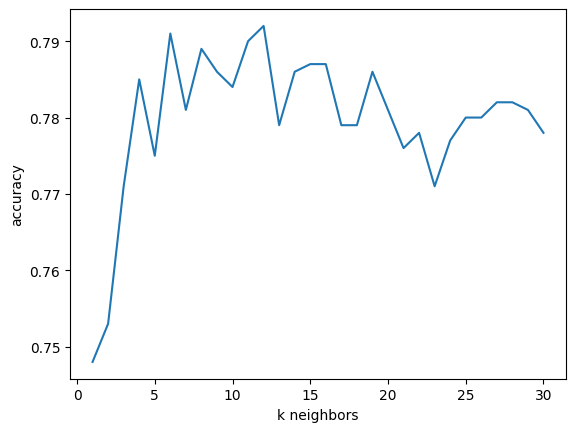
\includegraphics[scale=0.5]{./figures/output.png}
    \caption{The final result of \textbf{main()}}
\end{figure}

In my algorithm, the optimal number of neighbors is 12, with a cross-validation accuracy of 0.792. For the test set, it resulted in an accuracy of 0.7545.

\end{document}